In this section we will now test the accuracy and the performance of our Inverse Power Method with Deflation algorithm against the \texttt{eigs} function that is natively implemented in MATLAB. As perviously stated our objective is to compute the \(K\) smallest eigenvalues of a symmetric positive semidefinite matrix \(L\).
\\
\\
As benchmark matrix we now use the Laplacian matrix relative to the \texttt{circle} K-NN graph with \(K=10\). For the first benchmark run we computed the 15 smallest eigenvalues and eigenvector using the \texttt{eigs} function in MATLAB and the Inverse power method implemented by us using both the naive deflation method and the Wielandt's deflation method.
\begin{figure}[H]
    \centering
    \subfloat[1][Eigenvalues comparison]{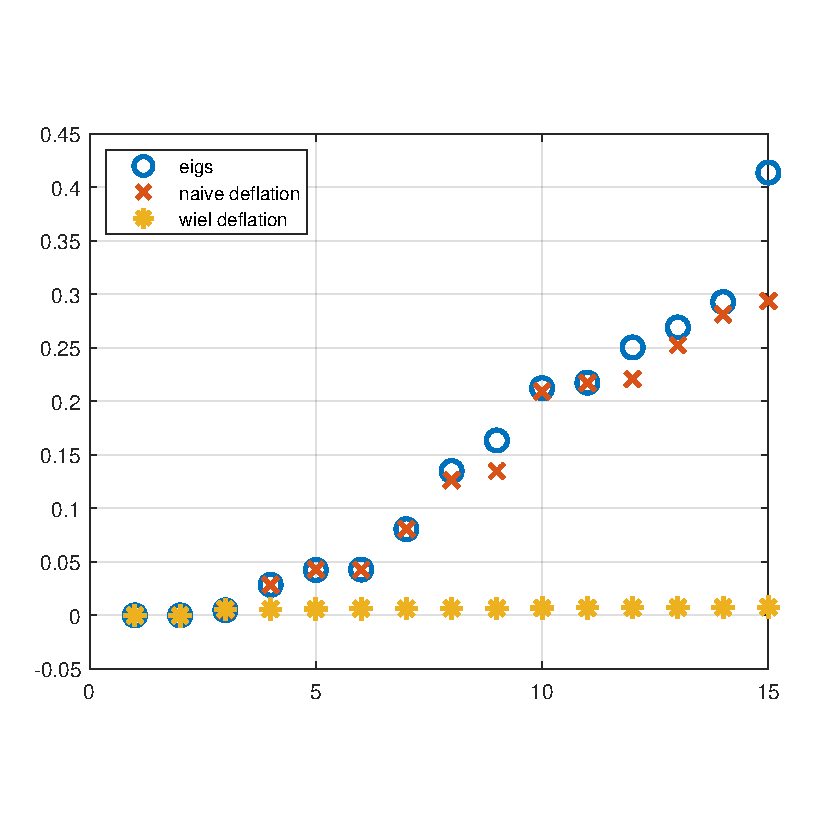
\includegraphics[scale = 0.5]{pictures/ipmd_test/eigenvalues_comp.pdf}}
    \subfloat[2][Partial times to compute eigenvalues in seconds]{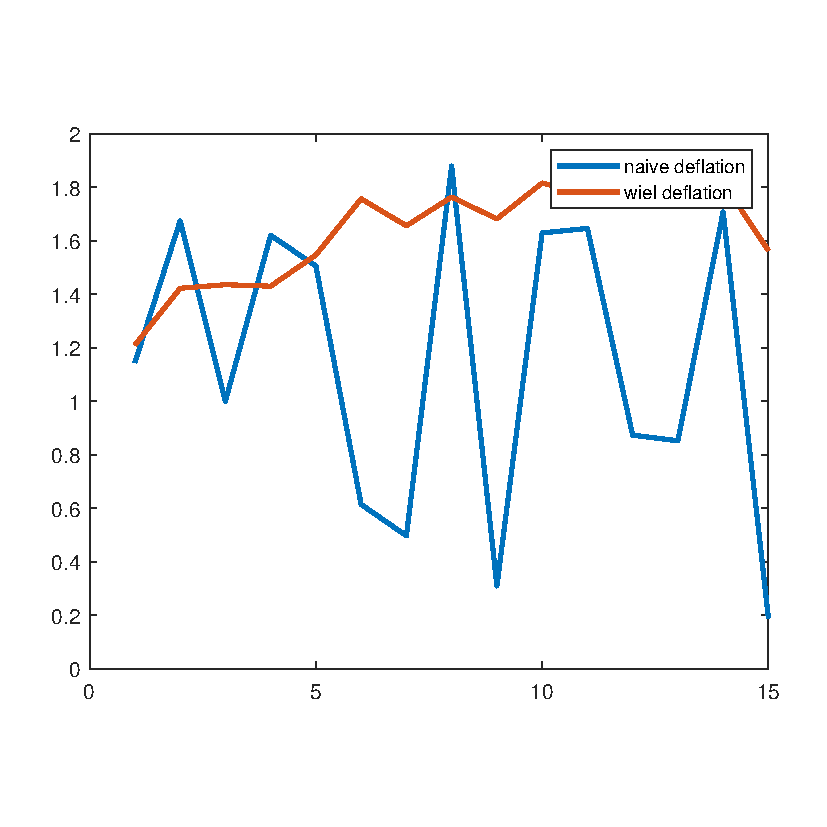
\includegraphics[scale = 0.5]{pictures/ipmd_test/times.pdf}}
    \caption{On the left the comparison between the values of the eigenvalues computed using all methods shown. On the right a plot of the partial times to compute each eigenvalue by using the inverse power method with deflation.}
    \label{Eigenvalues_comp}
\end{figure}

\begin{figure}[H]
    \centering
    \subfloat[1][\(u_1\)]{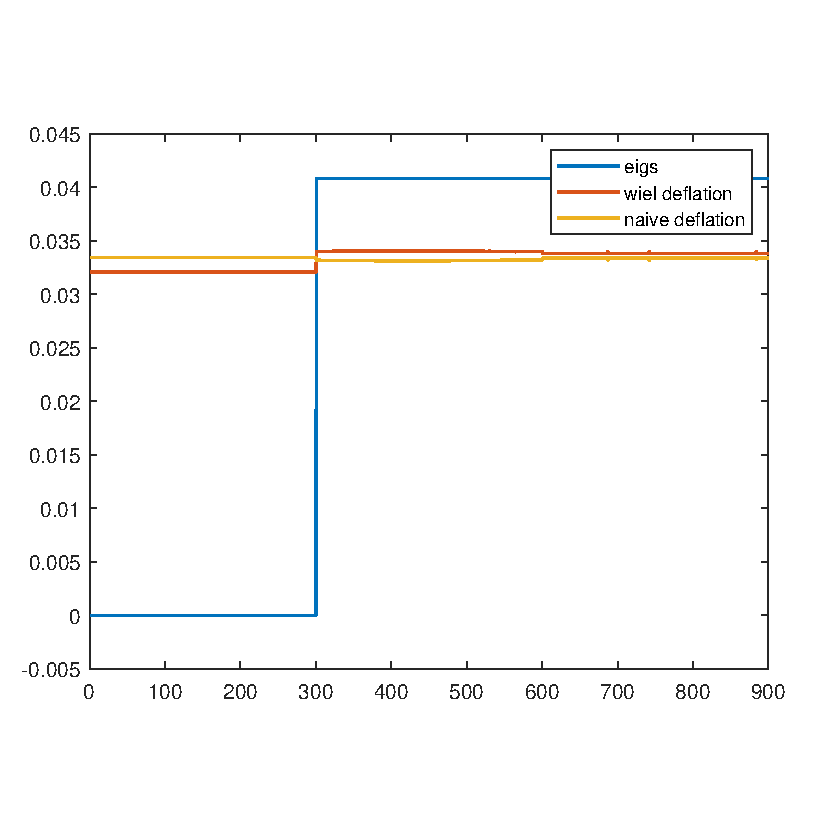
\includegraphics[scale = 0.35]{pictures/ipmd_test/eigenvector_1.pdf}}
    \subfloat[2][\(u_2\)]{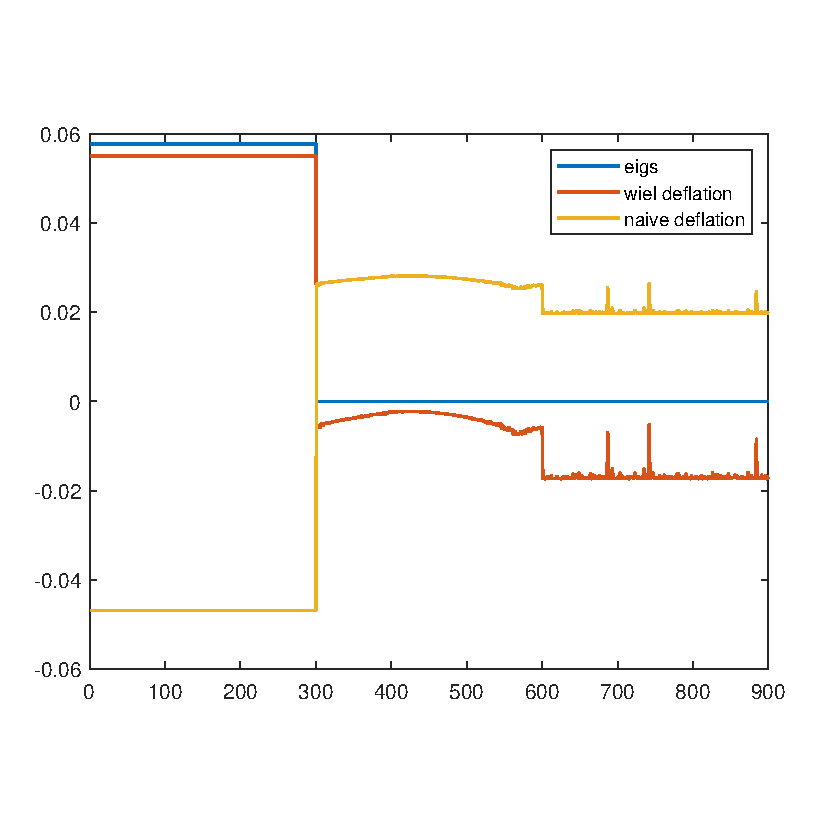
\includegraphics[scale = 0.35]{pictures/ipmd_test/eigenvector_2.pdf}}
    \subfloat[2][\(u_3\)]{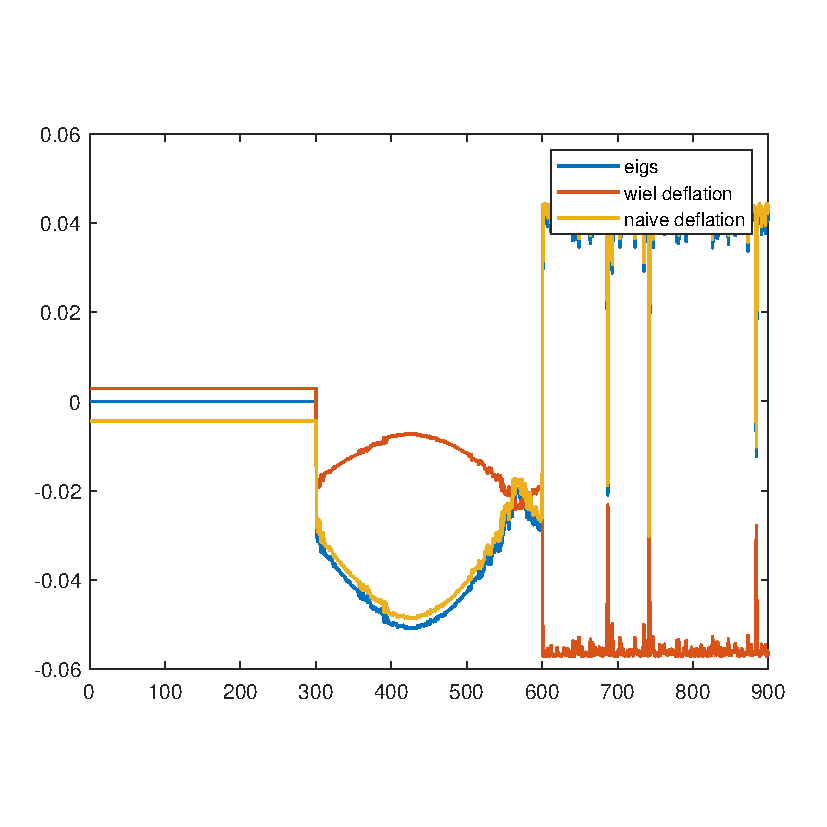
\includegraphics[scale = 0.35]{pictures/ipmd_test/eigenvector_3.pdf}}
    \caption{A plot of the first three eigenvectors computed using the three methods}
    \label{Eigenvectors_comp}
\end{figure}

TODO COMMENTARE RISULTATI

\subsection*{Using the normalized Laplacian matrix}
Using the normalized Laplacian matrix \(L_{\text{sym}} = I - D^{-\frac{1}{2}}WD^{-\frac{1}{2}}\) means that we are shrinking the spectrum of our matrix. We hence expect different results in terms of accuracy of the eigenvalues due to a smaller numerical error since we are comparing at each step numbers in the same order of magnitude.

\begin{figure}[H]
    \centering
    \subfloat[1][Eigenvalues comparison]{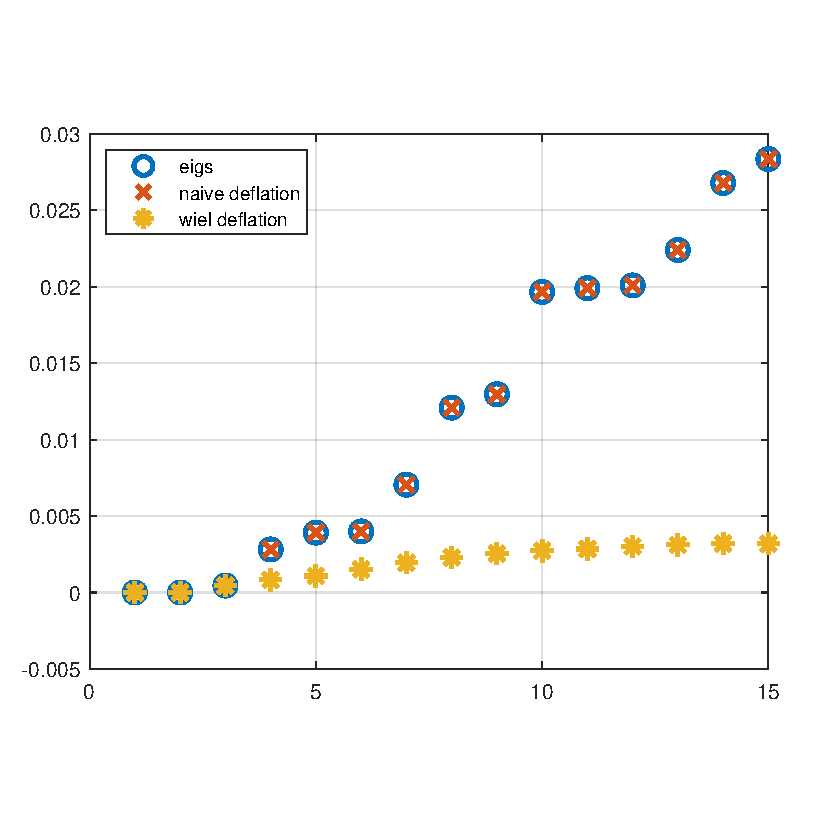
\includegraphics[scale = 0.5]{pictures/ipmd_test/eigenvalues_comp_norm.pdf}}
    \subfloat[2][Partial times to compute eigenvalues in seconds]{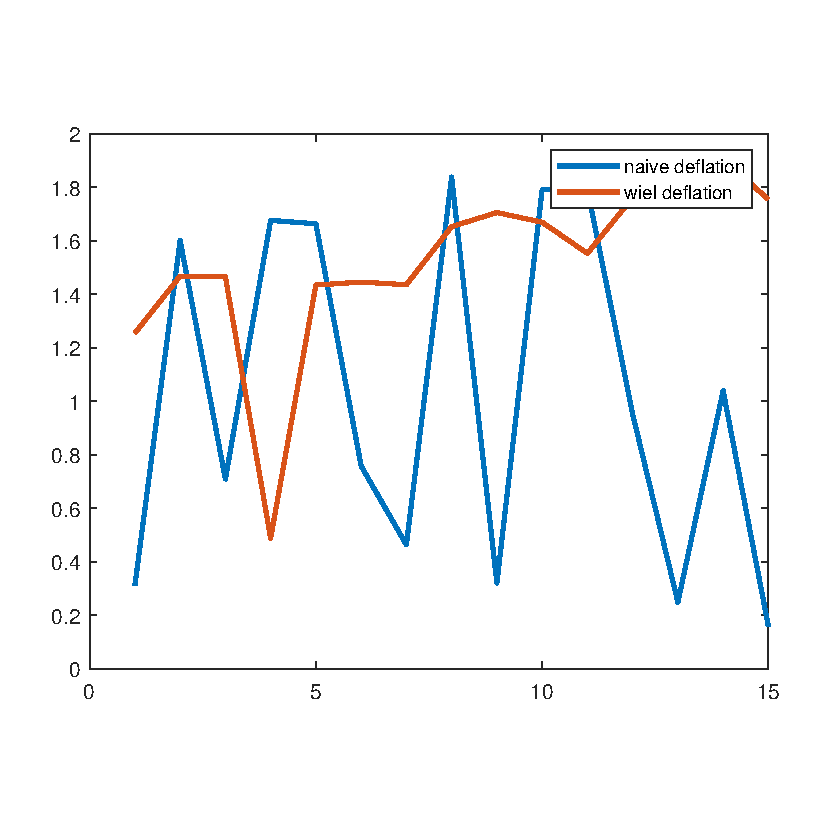
\includegraphics[scale = 0.5]{pictures/ipmd_test/times_norm.pdf}}
    \caption{On the left the comparison between the values of the eigenvalues computed using all methods shown. On the right a plot of the partial times to compute each eigenvalue by using the inverse power method with deflation.}
    \label{Eigenvalues_comp_norm}
\end{figure}

\begin{figure}[H]
    \centering
    \subfloat[1][\(u_1\)]{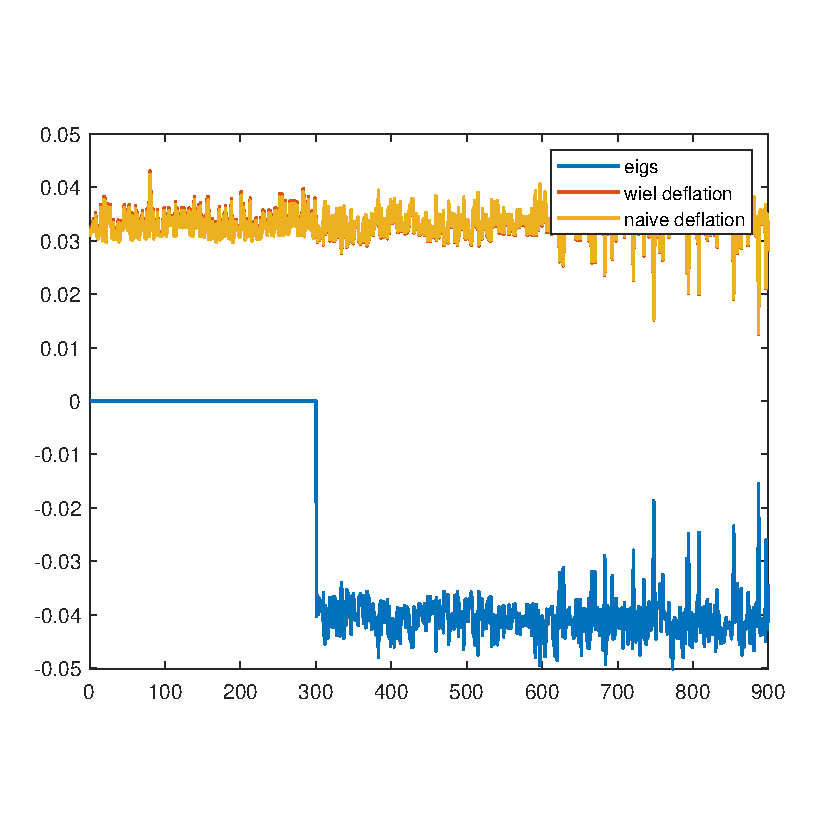
\includegraphics[scale = 0.35]{pictures/ipmd_test/eigenvector_norm_1.pdf}}
    \subfloat[2][\(u_2\)]{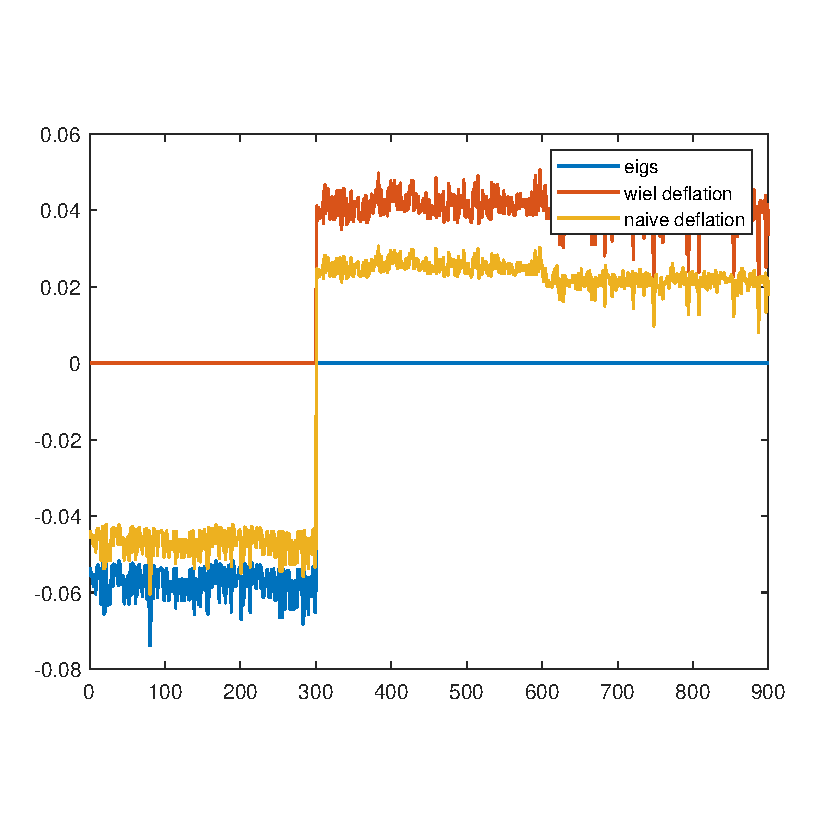
\includegraphics[scale = 0.35]{pictures/ipmd_test/eigenvector_norm_2.pdf}}
    \subfloat[2][\(u_3\)]{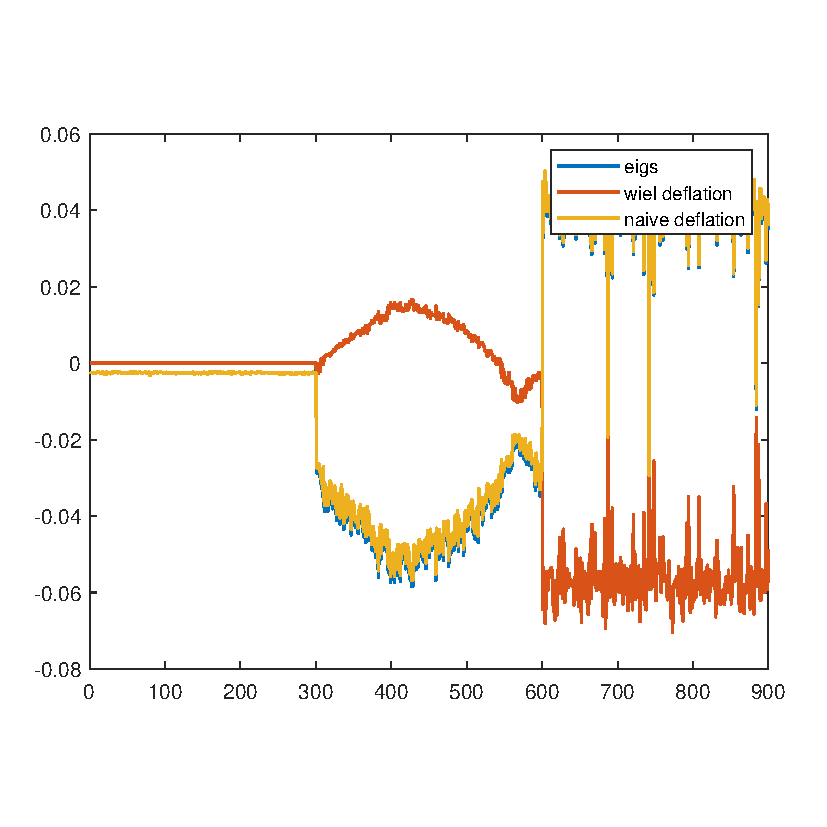
\includegraphics[scale = 0.35]{pictures/ipmd_test/eigenvector_norm_3.pdf}}
    \caption{A plot of the first three eigenvectors computed using the three methods}
    \label{Eigenvectors_comp_norm}
\end{figure}

TODO COMMENTARE RISULTATI.